\chapter*{Appendix}
\addcontentsline{toc}{chapter}{Appendix}

\section*{About the project}
\newthought{Lonnrot Scheme} was developed as a final project for a compiler design and implementation
course. In this section, we touch upon what we set out to do, how we went about doing it
and a brief overview of the project's timeline.

% a.1
\subsection*{Purpose, Scope and Inspiration}
\newthought{The purpose of this project} was to explore the design and implementation of a minimal
language that had \textit{Turing Completeness}. Naturally, however, this is
a very broad description: in the case of a functional language, having \texttt{lambda} suffices
to meet this criterion. In that sense, it is important to note that the project was meant to have
other operations, which I outline in the Requirements~\ref{app:reqs}. In this section, rather,
I'd like to elucidate the scope of the project\marginnote{A euphemism for ``justify my shortcomings''}
and talk about what made me try it out.

The original idea was for Lonnrot to also include the core of miniKanren. The value proposition
was to have miniKanren be compiled rather than interpreted, since it's something that has
not been done before. However, life got in the way and I was only able to (marginally) implement
the Scheme part of the whole affair. In any case, the inspiration for my workflow was given by
Abdulaziz Ghuloum in \textit{An Incremental Approach to Compiler Construction}.
\marginnote{Lindsey Kuper \cite{kuper19} talks about this approach and Kent Dybvig's
  ``cousin'' approach of writing the compiler back-to-front, making a language progressively more
  high-level, for those interested.}
The main idea is to write multiple compilers, with each one covering a progressively larger language.
This is opposed to the idea of writing one compiler, front to back, for the originally intended
language.

This has, amongst other implications, the effect of guiding my efforts towards making stuff work
for x86. Notably, there are no floats implemented in Lonnrot: since this was a semester long course
and parsing, execution and other things were also a priority (as opposed to Dybvig's course), it
followed that fiddling with bit representations of floats was a bit beyond the scope of the book
at best, and an exercise in frustration at worst. Likewise, error reporting in Lonnrot is weaker
compared to other (static) projects in the class, since it would have consumed too much time for
marginal gains grade-wise. It is, of course, my wish to keep hacking away at it on the long term,
hopefully incorporating things to make it more well-rounded and usable (or at least somewhat clearer
for educational purposes; it'd be nice to contribute to the a86 repository).

% a.2
\subsection*{Requirements}\label{app:reqs}
\newthought{In a very broad sense}, the project was required to achieve \textit{Turing Completeness}. More
specifically, being a functional language, Lonnrot Scheme was required to have at least:

\begin{itemize}
  \item Binding forms, assignment: \texttt{let}, \texttt{letrec}
  \item Conditionals: \texttt{if}, \texttt{cond}
  \item Math expressions, logical and relational operators: \texttt{+, -, *}, \texttt{<, >, =}
  \item Modules, functions: \texttt{define}, \texttt{letrec}, \texttt{lambda}
  \item Structured element: \texttt{cons}, \texttt{box}, \textbf{strings}
\end{itemize}

% a.3
\subsection*{Weekly Log}
\newthought{As described in the earlier appendix}, the point of following Ghuloum's and Dybvig's ideas was to
iteratively refine and grow the final compiler. As such, each entry of the log below can be understood as the
process of, roughly speaking:

\begin{itemize}
  \item Adding a node to the AST
  \item Adding a clause to \texttt{parse.rkt} and \texttt{mparse.rkt}
  \item Adding appropriate code to \texttt{interp.rkt} and \texttt{compile.rkt}
  \item Modifying the runtime if necessary
\end{itemize}

\begin{center}
	\begin{tabular}{@{}l|l@{}}
	      \toprule
	      \textbf{Week} & \textbf{Progress} \\
	      \midrule
	      Week 1 (April 7th)  & \parbox[c]{10cm}{Implemented integers and primitives \\ (\texttt{add1}, \texttt{sub1}, arithmetic \texttt{if})} \\[20pt]
	      Week 2 (April 14th) & \parbox[c]{10cm}{Implemented booleans, boolean \texttt{if}} \\[20pt]
	      Week 3 (April 21st) & \parbox[c]{10cm}{Implemented chars} \\[20pt]
	      Week 4 (April 28th) & \parbox[c]{10cm}{Implemented basic byte I/O, runtime exceptions} \\[20pt]
	      Week 5 (May 5th)    & \parbox[c]{10cm}{Implemented \texttt{let} and binary primitives such as \\ \texttt{+} and \texttt{-}} \\[20pt]
	      Week 6 (May 12th)   & \parbox[c]{10cm}{Implemented inductive data (\texttt{box}, \texttt{cons}) and \\ non first-class functions} \\[20pt]
	      Week 7 (May 19th)   & \parbox[c]{10cm}{Implemented TCO, \texttt{letrec} and \texttt{lambdas}} \\[20pt]
	      Week 8 (May 26th)   & \parbox[c]{10cm}{Implemented desugaring, added standard lib and amenities} \\[20pt]
	      Week 9 (June 2nd)   & \parbox[c]{10cm}{Finished documentation, added bells and whistles} \\[20pt]
	     \bottomrule
	\end{tabular}
\end{center}

\subsection*{Commit History}
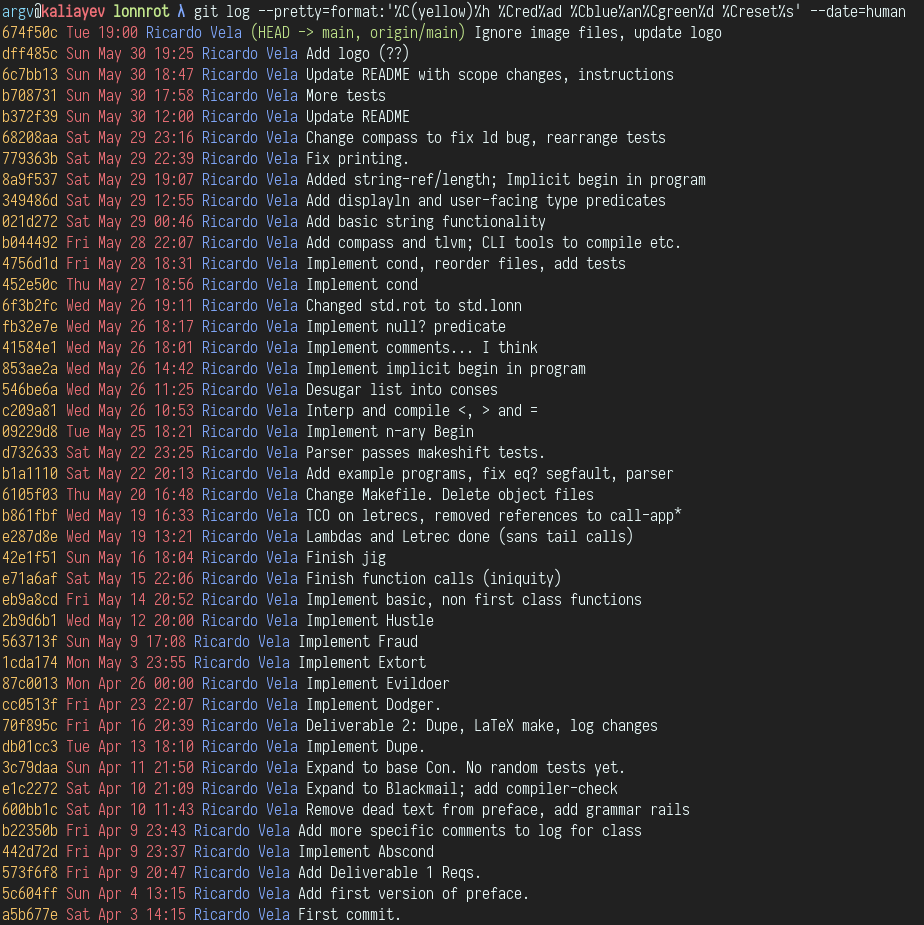
\includegraphics[width=0.8\paperwidth]{figures/appendix/git-log}


% c.1
\section*{Libraries and other Tooling}
\newthought{Lonnrot Scheme} is written in Racket. However, there are other parts of
the project that may warrant a more specific description of the tooling required in the project.

\begin{itemize}
  \item \textbf{Parsing:} \texttt{megaparsack} was used for parsing. Notable dependencies include
        \texttt{data/monad} and \texttt{data/applicative}, which allow the generation of symbolic
        expressions upon the successful application of a parser combinator.
  \item \textbf{AST Transformations:} For facilities when dealing with representing x86 instructions
        with Racket structs, \texttt{a86} was used.
  \item \textbf{Runtime:} As stated in the installation instructions in the Reference~\ref{p:2}, the
        runtime was written in C, and we depend on \texttt{nasm} and \texttt{gcc} to compile and link
        the object files of both a Lonnrot program and the runtime.
\end{itemize}

Lastly, Lonnrot Scheme was developed in Arch Linux.\marginnote{I swear this is not a ``btw i use arch'' joke}
